% !TEX TS-program = knitr
\documentclass[handout]{beamer}\usepackage{graphicx, color}
%% maxwidth is the original width if it is less than linewidth
%% otherwise use linewidth (to make sure the graphics do not exceed the margin)
\makeatletter
\def\maxwidth{ %
  \ifdim\Gin@nat@width>\linewidth
    \linewidth
  \else
    \Gin@nat@width
  \fi
}
\makeatother

\definecolor{fgcolor}{rgb}{0.2, 0.2, 0.2}
\newcommand{\hlnumber}[1]{\textcolor[rgb]{0,0,0}{#1}}%
\newcommand{\hlfunctioncall}[1]{\textcolor[rgb]{0.501960784313725,0,0.329411764705882}{\textbf{#1}}}%
\newcommand{\hlstring}[1]{\textcolor[rgb]{0.6,0.6,1}{#1}}%
\newcommand{\hlkeyword}[1]{\textcolor[rgb]{0,0,0}{\textbf{#1}}}%
\newcommand{\hlargument}[1]{\textcolor[rgb]{0.690196078431373,0.250980392156863,0.0196078431372549}{#1}}%
\newcommand{\hlcomment}[1]{\textcolor[rgb]{0.180392156862745,0.6,0.341176470588235}{#1}}%
\newcommand{\hlroxygencomment}[1]{\textcolor[rgb]{0.43921568627451,0.47843137254902,0.701960784313725}{#1}}%
\newcommand{\hlformalargs}[1]{\textcolor[rgb]{0.690196078431373,0.250980392156863,0.0196078431372549}{#1}}%
\newcommand{\hleqformalargs}[1]{\textcolor[rgb]{0.690196078431373,0.250980392156863,0.0196078431372549}{#1}}%
\newcommand{\hlassignement}[1]{\textcolor[rgb]{0,0,0}{\textbf{#1}}}%
\newcommand{\hlpackage}[1]{\textcolor[rgb]{0.588235294117647,0.709803921568627,0.145098039215686}{#1}}%
\newcommand{\hlslot}[1]{\textit{#1}}%
\newcommand{\hlsymbol}[1]{\textcolor[rgb]{0,0,0}{#1}}%
\newcommand{\hlprompt}[1]{\textcolor[rgb]{0.2,0.2,0.2}{#1}}%

\usepackage{framed}
\makeatletter
\newenvironment{kframe}{%
 \def\at@end@of@kframe{}%
 \ifinner\ifhmode%
  \def\at@end@of@kframe{\end{minipage}}%
  \begin{minipage}{\columnwidth}%
 \fi\fi%
 \def\FrameCommand##1{\hskip\@totalleftmargin \hskip-\fboxsep
 \colorbox{shadecolor}{##1}\hskip-\fboxsep
     % There is no \\@totalrightmargin, so:
     \hskip-\linewidth \hskip-\@totalleftmargin \hskip\columnwidth}%
 \MakeFramed {\advance\hsize-\width
   \@totalleftmargin\z@ \linewidth\hsize
   \@setminipage}}%
 {\par\unskip\endMakeFramed%
 \at@end@of@kframe}
\makeatother

\definecolor{shadecolor}{rgb}{.97, .97, .97}
\definecolor{messagecolor}{rgb}{0, 0, 0}
\definecolor{warningcolor}{rgb}{1, 0, 1}
\definecolor{errorcolor}{rgb}{1, 0, 0}
\newenvironment{knitrout}{}{} % an empty environment to be redefined in TeX

\usepackage{alltt}
\newcommand{\answers}{1}


\usetheme{Marburg}
\setbeamertemplate{navigation symbols}{} 
\setbeamertemplate{footline}
{
  \leavevmode%
  \hbox{%
  \begin{beamercolorbox}[wd=.333333\paperwidth,ht=2.25ex,dp=1ex,center]{author in head/foot}%
    \usebeamerfont{author in head/foot}\copyright $\ $ \insertshortauthor%~~\beamer@ifempty{\insertshortinstitute}{}{(\insertshortinstitute)}
  \end{beamercolorbox}%
  \begin{beamercolorbox}[wd=.333333\paperwidth,ht=2.25ex,dp=1ex,center]{title in head/foot}%
    \usebeamerfont{title in head/foot} \insertinstitute
  \end{beamercolorbox}%
  \begin{beamercolorbox}[wd=.333333\paperwidth,ht=2.25ex,dp=1ex,right]{date in head/foot}%
    \usebeamerfont{date in head/foot}\insertshortdate{}\hspace*{2em}
    \insertframenumber{} / \inserttotalframenumber\hspace*{2ex} 
  \end{beamercolorbox}}%
  \vskip0pt%
}

\usepackage{amsmath}
\usepackage{caption}
\usepackage{color}
\usepackage{enumerate}
\usepackage{listings}
\usepackage{hyperref}
\usepackage{mathrsfs}
\usepackage{natbib}
\usepackage{url}
\usepackage{mdwlist}

\providecommand{\all}{\ \forall \ }
\providecommand{\bs}{\backslash}
\providecommand{\e}{\varepsilon}
\providecommand{\E}{\ \exists \ }
\providecommand{\lm}[2]{\lim_{#1 \rightarrow #2}}
\providecommand{\m}[1]{\mathbb{#1}}
\providecommand{\nv}{{}^{-1}}
\providecommand{\ov}[1]{\overline{#1}}
\providecommand{\p}{\newpage}
\providecommand{\q}{$\quad$ \newline}
\providecommand{\rt}{\rightarrow}
\providecommand{\Rt}{\Rightarrow}
\providecommand{\vc}[1]{\boldsymbol{#1}}
\providecommand{\wh}[1]{\widehat{#1}}

\hypersetup{colorlinks,linkcolor=,urlcolor=blue}
\numberwithin{equation}{section}

\definecolor{dkgreen}{rgb}{0,0.6,0}
\definecolor{gray}{rgb}{0.5,0.5,0.5}
\definecolor{mauve}{rgb}{0.58,0,0.82}

\lstset{ 
  language=C,                % the language of the code
  basicstyle= \footnotesize,           % the size of the fonts that are used for the code
  numberstyle= \tiny \color{white},  % the style that is used for the line-numbers
  stepnumber=2,                   % the step between two line-numbers. 
  numbersep=5pt,                  % how far the line-numbers are from the code
  backgroundcolor=\color{white},      % choose the background color. You must add \usepackage{color}
  showspaces=false,               % show spaces adding particular underscores
  showstringspaces=false,         % underline spaces within strings
  showtabs=false,                 % show tabs within strings adding particular underscores
  frame=lrb,                   % adds a frame around the code
  rulecolor=\color{black},        % if not set, the frame-color may be changed on line-breaks within not-black text 
  tabsize=2,                      % sets default tabsize to 2 spaces
  captionpos=t,                   % sets the caption-position 
  breaklines=true,                % sets automatic line breaking
  breakatwhitespace=false,        % sets if automatic breaks should only happen at whitespace
  %title=\lstname,                   % show the filename of files included with \lstinputlisting;
  keywordstyle=\color{blue},          % keyword style
  commentstyle=\color{gray},       % comment style
  stringstyle=\color{dkgreen},         % string literal style
  escapeinside={\%*}{*)},            % if you want to add LaTeX within your code
  morekeywords={*, ...},               % if you want to add more keywords to the set
  xleftmargin=0.053in, % left horizontal offset of caption box
  xrightmargin=-.03in % right horizontal offset of caption box
}

%\DeclareCaptionFont{white}{\color{white}}
%\DeclareCaptionFormat{listing}{\parbox{\textwidth}{\colorbox{gray}{\parbox{\textwidth}{#1#2#3}}\vskip-0.05in}}
%\captionsetup[lstlisting]{format = listing, labelfont = white, textfont = white}
%For caption-free listings, comment out the 3 lines above and uncomment the 2 lines below.
 \captionsetup{labelformat = empty, labelsep = none}
 \lstset{frame = single}




\title{Hypothesis Testing (Ch. 6.2)}
\author{Will Landau}
\date{Apr 2, 2013}
\institute{Iowa State University}
\IfFileExists{upquote.sty}{\usepackage{upquote}}{}

\begin{document}

\begin{frame}
\titlepage
 \end{frame}
 
 \AtBeginSection[]
{
   \begin{frame}
       \frametitle{Outline}
       \tableofcontents[currentsection]
   \end{frame}
}

\section{A review of Hypothesis Testing with Confidence Intervals}

\begin{frame}
\frametitle{Statistical inference}
\begin{itemize}
\item {\bf Statistical inference}: using data from the sample to draw conclusions about the population 
\begin{itemize}
\pause \item Point estimation (confidence intervals): estimating population parameters and specifying the degree of precision of the estimate.
\pause \item Hypothesis testing: testing the validity of statements about the population that are framed in terms of parameters. 
\end{itemize}
\end{itemize}
\end{frame}

\begin{frame}
\frametitle{Hypothesis testing} \scriptsize
\begin{itemize}
\item {\bf Hypothesis testing (significance testing)}: the use of data in the quantitative assessment of the plausibility of some trial value or a parameter. 
\pause \item You have competing {\bf hypotheses}, or statements, about a population:
\begin{itemize}
\pause \item The {\bf null hypothesis}, denoted $H_0$ is the proposition that a parameter equals some fixed number.
\pause \item The {\bf alternative hypothesis}, denoted $H_a$ or $H_1$, is a statement that stands in opposition to the null hypothesis.
\pause \item Examples:\q
\setkeys{Gin}{width=.6\textwidth} 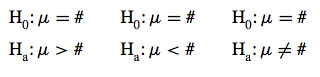
\includegraphics{../../fig/examplehypotheses.png}
\end{itemize}
\pause \item Note: $H_a: \mu \ne \#$ makes a {\bf two-sided test}, while $H_a: \mu < \#$ and $H_a: \mu > \#$ make a {\bf one-sided test}.
\pause \item The goal is to use the data to debunk the null hypothesis in favor of the alternative:
\begin{itemize}
\pause \item Assume $H_0$.
\pause \item Try to show that, under $H_0$, the data are preposterous.
\pause \item If the data are preposterous, reject $H_0$ and conclude $H_a$. Otherwise, fail to reject $H_0$.
\end{itemize}
\end{itemize}
\end{frame}

\begin{frame}
\frametitle{Hypothesis testing}
\begin{itemize}
\item Outcomes of a hypothesis test: \q
\setkeys{Gin}{width=.5\textwidth} 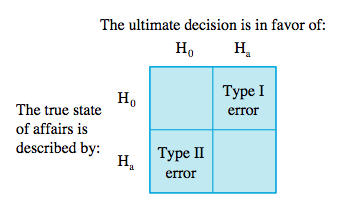
\includegraphics{../../fig/typeerrors.png}
\pause \item $\alpha$ (the very same $\alpha$ in confidence intervals) is the probability of rejecting $H_0$ when $H_0$ is true.
\begin{itemize}
\pause \item $\alpha$ is the Type I Error probability.
\pause \item For honesty's sake, $\alpha$ is fixed before you even \emph{look} at the data.
\end{itemize} 
\end{itemize}
\end{frame}

\begin{frame}
\frametitle{Formal steps of a hypothesis test using confidence intervals}
\begin{enumerate}[1. ]
\item State $H_0$ and $H_a$.
\pause \item State $\alpha$.
\pause \item State the form of the $1 - \alpha$ confidence interval you will use, along with all the assumptions necessary.
\pause \item Calculate the $1 - \alpha$ confidence interval.
\pause \item Based on the $1 - \alpha$ confidence interval, either:
\begin{itemize}
\pause \item Reject $H_0$ and conclude $H_a$, or
\pause \item Fail to reject $H_0$.
\end{itemize}
\pause \item Interpret the conclusion using layman's terms.
\end{enumerate}
\end{frame}


\begin{frame}
\frametitle{Example: breaking strength of wire}
\begin{itemize}
\item Suppose you are a manufacturer of construction equipment. You make 0.0125 inch wire rope and need to determine how much weight it can hold before breaking so that you can label it clearly.
\pause \item Here are breaking strengths, in kg, for 40 sample wires:
\end{itemize}
\setkeys{Gin}{width=1\textwidth} 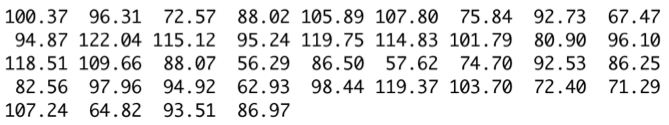
\includegraphics{../../fig/wiredata.png}
\begin{itemize}
\pause \item Let's conduct a hypothesis test to find out if the true mean breaking strength is above 85 kg.
\end{itemize}
\end{frame}

\begin{frame}
\frametitle{Example: breaking strength of wire} \scriptsize
\begin{enumerate}[1. ]
\item $H_0: \mu = 85$ kg and $H_a: \mu > 85$ kg, where $\mu$ is the true mean breaking strength.
\pause \item $\alpha$ = 0.05
\pause \item Since this is a one-sided (lower) test, I will use a lower $1 - \alpha$ confidence interval:
\begin{align*}
\left (\ov{x} - z_{1 - \alpha} \frac{s}{\sqrt{n}}, \ \infty \right )
\end{align*}
\pause I am assuming:
\begin{itemize}
\pause \item The data points $x_1, \ldots x_n$ were iid draws from some distribution with mean $\mu$ and some constant variance.
\end{itemize}
\pause \item From before, we calculated the confidence interval to be $(87.24, \infty)$.
\pause \item With 95\% confidence, we have shown that $\mu > 87.24$. Hence, at significance level $\alpha = 0.05$, we have shown that $\mu > 85$. We reject $H_0$ and conclude $H_a$.
\pause \item There is enough evidence to conclude that the true mean breaking strength of the wire is greater than 85 kg. Hence, the requirement is met.
\end{enumerate}
\end{frame}

\section{Hypothesis Testing with Critical Values}

\begin{frame}
\frametitle{Hypothesis testing with critical values}
\begin{itemize}
\item Instead of using a confidence interval in the test, simply compute a test statistic and compare it to a {\bf critical value}.
\pause \item A {\bf test statistic} is a number of the form: 
\begin{align*}
K = \frac{\ov{x} - \mu_0}{\phi}
\end{align*}
\begin{itemize}
\pause \item $\mu_0$ is the true mean value of the data under the null hypothesis.
\pause \item $\phi$ is either $\sigma/\sqrt{n}$ or $s/\sqrt{n}$, whichever version of $SD(\ov{X})$ is available.
\end{itemize}
\pause \item A {\bf critical value} is a special quantile on the distribution of $K$ (either $z_{1 - \alpha}$, $z_{1 - \alpha/2}$, $t_{n - 1, 1 - \alpha}$, or $t_{n - 1, 1 - \alpha/2}$). We compare it to $K$ to decide whether to reject $H_0$ or fail to reject $H_0$.
\end{itemize}
\end{frame}


\begin{frame}
\frametitle{Full list of steps: critical values}
\begin{enumerate}[1. ]
\item State $H_0$ and $H_a$.
\pause \item State $\alpha$.
\pause \item State the form of the test statistic, its distribution under the null hypothesis, and all your assumptions.
\pause \item Calculate the test statistic and the critical value
\pause \item Based on the previous step, either:
\begin{itemize}
\pause \item Reject $H_0$ and conclude $H_a$, or
\pause \item Fail to reject $H_0$.
\end{itemize}
\pause \item Interpret the conclusion using layman's terms.
\end{enumerate}
\end{frame}






\begin{frame}
\frametitle{Example: fill weight of jars} \small
\begin{itemize}
\pause \item Suppose a manufacturer fills jars of food using a stable filling process with a known standard deviation of $\sigma = 1.6 g$. 
\pause \item We take a sample of $n = $47 jars and measure the sample mean weight $\ov{x} = 138.2$ g.
\pause \item I will conduct the following hypothesis tests:
\begin{itemize}
\pause \item $H_0: \mu = 140$ vs. $H_a: \mu \ne 140$
\pause \item $H_0: \mu = 138$ vs. $H_a: \mu < 138$
\end{itemize}
\end{itemize}
\end{frame}

\begin{frame}
\frametitle{ $H_0: \mu = 140$ vs. $H_a: \mu \ne 140$} \small

\begin{enumerate}[1. ]
\item  $H_0: \mu = 140$, $H_a: \mu \ne 140$
\pause \item $\alpha = 0.1$
\pause \item Since $\sigma$ is known and the sample size is large enough for the Central Limit Theorem, I will use the test statistic:
\begin{align*}
K = \frac{\ov{x} - 140}{\sigma/\sqrt{n}}
\end{align*}
\begin{itemize}
\pause \item Assume $X_1, \ldots, X_n$ are iid with mean $\mu$ and variance $\sigma^2$.
\pause \item $K \sim N(0,1)$ under the null hypothesis.
\pause \item Since $K \sim N(0,1)$ and this is a 2-sided test, I reject $H_0$ when $|K| > |z_{1 - \alpha/2}|$.
\end{itemize}

\end{enumerate}
\end{frame}


\begin{frame}[fragile]
\frametitle{ $H_0: \mu = 140$ vs. $H_a: \mu \ne 140$} \small
\begin{itemize}
\item {\bf Rejection region}: the set of all possible values of $K$ for which the $H_0$ is rejected.
\pause \item The pdf of $K$ must integrate to $\alpha$ over the rejection region (in this case, $(-\infty, z_{\alpha/2})$ and $(z_{1-\alpha/2}, \ \infty)$).
\end{itemize}
\pause \begin{center}
\begin{knitrout}
\definecolor{shadecolor}{rgb}{0.969, 0.969, 0.969}\color{fgcolor}
\includegraphics[width=0.6\textwidth,height=0.6\textheight]{figure/unnamed-chunk-2} 

\end{knitrout}

\end{center}
\end{frame}

\begin{frame}
\frametitle{ $H_0: \mu = 140$ vs. $H_a: \mu \ne 140$} \small
\begin{enumerate}
\setcounter{enumi}{3}
\item The moment of truth:
\begin{itemize}
\pause \item \[K = \frac{138.2 - 140}{1.6/\sqrt{47}} = -7.72\]
\pause \item $z_{1-\alpha/2} = z_{1-0.1/2} = z_{0.95} = 1.64$.
\end{itemize}
\pause \item Since $|K| = |-7.72| > 1.64 = |z_{1 - \alpha/2}|$, I reject $H_0$ in favor of $H_a$.
\pause \item There is strong evidence that the true mean fill weight is not 140 g.
\end{enumerate}
\end{frame}







\begin{frame}
\frametitle{ $H_0: \mu = 138$ vs. $H_a: \mu < 138$} \small
\begin{enumerate}[1. ]
\item  $H_0: \mu = 138$, $H_a: \mu < 138$
\pause \item $\alpha = 0.1$
\pause \item Since $\sigma$ is known and the sample size is large enough for the Central Limit Theorem, I will use the test statistic:
\begin{align*}
K = \frac{\ov{x} - 138}{\sigma/\sqrt{n}}
\end{align*}
\begin{itemize}
\pause \item Assume $X_1, \ldots, X_n$ are iid with mean $\mu$ and variance $\sigma^2$.
\pause \item $K \sim N(0,1)$ under the null hypothesis.
\pause \item Since $K \sim N(0,1)$ and this is a 1-sided upper test, I reject $H_0$ when $K < z_{\alpha}$.
\end{itemize}

\end{enumerate}
\end{frame}


\begin{frame}
\frametitle{ $H_0: \mu = 138$ vs. $H_a: \mu < 138$} \small
\begin{itemize}
\item This time, our rejection region is $(-\infty,\  z_{\alpha})$.
\pause \item The pdf of $K$ must integrate to $\alpha$ over the rejection region.
\end{itemize}
\pause \begin{center}
\begin{knitrout}
\definecolor{shadecolor}{rgb}{0.969, 0.969, 0.969}\color{fgcolor}
\includegraphics[width=0.6\textwidth,height=0.6\textheight]{figure/unnamed-chunk-3} 

\end{knitrout}


\end{center}
\end{frame}

\begin{frame}
\frametitle{ $H_0: \mu = 138$ vs. $H_a: \mu < 138$} \small
\begin{enumerate}
\setcounter{enumi}{3}
\item The moment of truth:
\begin{itemize}
\pause \item \[K = \frac{138.2 - 138}{1.6/\sqrt{47}} = 0.857\]
\pause \item $z_{\alpha} = z_{0.1} = -1.28$.
\end{itemize}
\pause \item Since $K = 0.857$, which is not less than $z_\alpha = -1.28$, I fail to reject $H_0$.
\pause \item There is not enough evidence to conclude that the true mean fill weight is less than 138 g.
\end{enumerate}
\end{frame}





\begin{frame}
\frametitle{Example: concrete beams}
\begin{itemize}
\item 10 concrete beams were each measured for flexural strength (MPa):
\pause \begin{center}
\setkeys{Gin}{width=.7\textwidth} 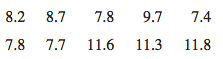
\includegraphics{../../fig/fbeams.png}
\end{center}
\pause \item $\ov{x} = 9.2$ MPa, $s = 1.76$ MPa.
\pause \item I will conduct a hypothesis test to find out if the flexural strength is above 8.0 MPa.
\end{itemize}
\end{frame}

\begin{frame}
\frametitle{Example: concrete beams}
\begin{enumerate}[1. ]
\item  $H_0: \mu = 8.0$, $H_a: \mu > 8.0$
\pause \item $\alpha = 0.05$
\pause \item Since the sample size is small, I will use the test statistic:
\begin{align*}
K = \frac{\ov{x} - 8.0}{s/\sqrt{n}}
\end{align*}
\begin{itemize}
\pause \item Assume $X_1, \ldots, X_n$ are iid $N(\mu, \sigma^2)$
\pause \item $K \sim t_{n - 1} = t_{9}$ under the null hypothesis because $n$ is small and $\sigma$ is unknown.
\pause \item Since $K \sim t_9$ and this is a 1-sided lower test, I reject $H_0$ when $K > t_{9, 1-\alpha}$.
\end{itemize}

\end{enumerate}
\end{frame}






\begin{frame}[fragile]
\frametitle{Example: concrete beams}
\begin{itemize}
\item This time, our rejection region is $( z_{1-\alpha}, \infty)$.
\pause \item The pdf of $K$ must integrate to $\alpha$ over the rejection region.
\end{itemize}
\pause \begin{center}
\begin{knitrout}
\definecolor{shadecolor}{rgb}{0.969, 0.969, 0.969}\color{fgcolor}
\includegraphics[width=0.6\textwidth,height=0.6\textheight]{figure/unnamed-chunk-4} 

\end{knitrout}


\end{center}
\end{frame}

\begin{frame}
\frametitle{Example: concrete beams}
\begin{enumerate}
\setcounter{enumi}{3}
\item The moment of truth:
\begin{itemize}
\pause \item \[K = \frac{9.2 -  8.0}{1.76/\sqrt{10}} = 2.16\]
\pause \item $z_{1-\alpha} = z_{0.95} = 1.64$.
\end{itemize}
\pause \item Since $K = 2.16 > z_\alpha = 1.64$, I reject $H_0$ in favor of $H_a$.
\pause \item There is enough evidence to conclude that the true mean flexural strength of the beams is above 8.0 MPa.
\end{enumerate}
\end{frame}


\begin{frame}
\frametitle{Which test statistics and critical values to use} \scriptsize
\begin{itemize}
\item The rules for test statistics depend on the sample size $n$ and the knowledge of $\sigma$ in the same way confidence intervals do.
\end{itemize}
\pause \begin{tabular}{c|cc}
Condition & Test Statistic $K$& Distribution of $K$ \\ \hline
$n \ge 25$, $\sigma$ known  & $\displaystyle \frac{\mu - \mu_0}{\sigma/\sqrt{n}} $& $N(0,1)$  \\ [2.5ex]
$n \ge 25$, $\sigma$ unknown  &  $\displaystyle \frac{\mu-\mu_0}{s/\sqrt{n}}$ & $N(0,1)$ \\ [2.5ex]
$n < 25$, $\sigma$ unknown  & $\displaystyle \frac{\mu-\mu_0}{s/\sqrt{n}}$ & $t_{n-1}$   \\ [2.5ex]
\end{tabular}
\begin{itemize}
\pause \item Appropriate comparisons of critical values with the test statistic:
\end{itemize}
\pause \begin{tabular}{c|lll}
 & $H_a: \mu \ne \mu_0$ & $H_a: \mu < \mu_0$ & $H_a: \mu > \mu_0$  \\ \hline
$n \ge 25, \sigma$ & $|K| > |z_{1- \alpha/2}| $& $K < z_{\alpha}$ & $K > z_{1-\alpha}$ \\ [2.5ex]
$n \ge 25, s$ & $|K| > |z_{1 - \alpha/2}| $ & $K < z_{\alpha}$ &  $K > z_{1-\alpha}$\\ [2.5ex]
$n < 25, s$    & $|K| > |t_{n - 1,\  1 - \alpha/2}|$ & $K < t_{n - 1,\ \alpha}$ &$K > t_{n - 1, \ 1- \alpha}$   \\ [2.5ex]
\end{tabular}
\end{frame}


\begin{frame}
\frametitle{Your turn: car engines}
\begin{itemize}
\item Consider a grinding process used to rebuild car engines, which involves grinding rod journals for engine crankshafts. 
\pause \item Of interest is the deviation of the true mean rod journal diameter from the target diameter.
\pause \item 32 consecutive rod journals are ground, with a sample mean deviation of $-0.16 \times 10^{-4}$ in from the target diameter.
\pause \item The sample standard deviation of these deviations is $s = 0.7 \times 10^{-4}$ in.
\pause \item At a significance level of $\alpha = 0.05$, conduct a hypothesis test to determine whether the rod journal diameters are significantly off target.
\end{itemize}
\end{frame}



\begin{frame}<handout:\answers>
\frametitle{Answers: car engines}
\begin{enumerate}[1. ]
\item  $H_0: \mu = 0$, $H_a: \mu \ne 0$. 
\pause \item $\alpha = 0.05$
\pause \item Since $\sigma$ is unknown, I use:
\begin{align*}
K = \frac{\ov{x} - 8.0}{s/\sqrt{n}}
\end{align*}
\begin{itemize}
\pause \item Assume $X_1, \ldots, X_n$ are iid $(\mu, \sigma^2)$. Since $n \ge 25$, they don't need to be normally distributed.
\pause \item $K \sim N(0,1)$ under the null hypothesis because $n \ge 25$.
\pause \item Since $K \sim N(0,1)$ and this is a 2-sided test, I reject $H_0$ when $|K| > |z_{1-\alpha/2}|$.
\end{itemize}
\end{enumerate}
\end{frame}


\begin{frame}<handout:\answers>
\frametitle{Answers: car engines}
\begin{enumerate}
\setcounter{enumi}{3}
\item The moment of truth:
\begin{itemize}
\pause \item $K = \frac{-0.16 \times 10^{-4} - 0}{0.7 \times 10^{-4}/\sqrt{32}} = -1.29 $
\pause \item $z_{1-\alpha/2} = z_{0.975} = 1.96$.
\end{itemize}
\pause \item Since $|K| = 1.29 \not > z_\alpha = 1.96$, I fail to reject $H_0$.
\pause \item There is not enough evidence to conclude that the rod journal diameters are off target.
\end{enumerate}
\end{frame}







\section{Hypothesis Testing with p-values}


\begin{frame}[fragile]
\frametitle{p-values}
\begin{itemize}
\item A {\bf p-value} is the probability of getting a result at least as extreme as the one observed under the null hypothesis.
\pause \item More specifically, it's the probability (assuming the null hypothesis is true) of observing a test statistic farther into the rejection region than $K$.
\end{itemize}

\pause \begin{center}

\begin{knitrout}
\definecolor{shadecolor}{rgb}{0.969, 0.969, 0.969}\color{fgcolor}
\includegraphics[width=0.6\textwidth,height=0.6\textheight]{figure/unnamed-chunk-5} 

\end{knitrout}

\end{center}
\end{frame}



\begin{frame}
\frametitle{Full list of steps: p-values}
\begin{enumerate}[1. ]
\item State $H_0$ and $H_a$.
\pause \item State $\alpha$.
\pause \item State the form of the test statistic, its distribution under the null hypothesis, and all your assumptions.
\pause \item Calculate the test statistic and the p-value
\pause \item Make a decision based on the p-value.
\begin{itemize}
\pause \item If the p-value $< \alpha$, reject $H_0$ and conclude $H_a$.
\pause \item Otherwise, fail to reject $H_0$.
\end{itemize}
\pause \item Interpret the conclusion using layman's terms.
\end{enumerate}
\end{frame}

\begin{frame}
\frametitle{Calculating p-values}
\begin{itemize}
\pause \item Let $K$ be the value of the test statistic, $Z \sim N(0,1)$, and $T \sim t_{n-1}$. Here is a table of p-values that you should use for each set of conditions and choice of $H_a$. \q
\end{itemize}
\pause \begin{tabular}{c|lll}
 & $H_a: \mu \ne \mu_0$ & $H_a: \mu < \mu_0$ & $H_a: \mu > \mu_0$  \\ \hline
$n \ge 25, \sigma$ & $P(|Z| > |K|)$ & $P(Z < K)$ & $P(Z > K)$ \\ [2.5ex]
$n \ge 25, s$ & $P(|Z| > |K|)$           & $P(Z < K)$ & $P(Z > K)$\\ [2.5ex]
$n < 25, s$    & $P(|T| > |K|)$           & $P(T < K)$ & $P(T > K)$   \\ [2.5ex]
\end{tabular}
\end{frame}















\begin{frame}
\frametitle{Example: concrete beams}
\begin{itemize}
\item 10 concrete beams were each measured for flexural strength (MPa):
\pause \begin{center}
\setkeys{Gin}{width=.7\textwidth} 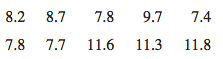
\includegraphics{../../fig/fbeams.png}
\end{center}
\pause \item $\ov{x} = 9.2$ MPa, $s = 1.76$ MPa.
\pause \item I will conduct a hypothesis test to find out if the flexural strength is different from 9.0 MPa.
\end{itemize}
\end{frame}


\begin{frame}
\frametitle{Example: concrete beams}
\begin{enumerate}[1. ]
\item  $H_0: \mu = 9.0$, $H_a: \mu \ne 9.0$
\pause \item $\alpha = 0.05$
\pause \item Since the sample size is small, I will use the test statistic:
\begin{align*}
K = \frac{\ov{x} - 9.0}{s/\sqrt{n}}
\end{align*}
\begin{itemize}
\pause \item Assume $X_1, \ldots, X_n$ are iid $N(\mu, \sigma^2)$
\pause \item $K \sim t_{n - 1} = t_{9}$ under the null hypothesis because $n$ is small and $\sigma$ is unknown.
\end{itemize}
\end{enumerate}
\end{frame}





\begin{frame}
\frametitle{Example: concrete beams}
\begin{enumerate}
\setcounter{enumi}{3}
\item The moment of truth:
\begin{itemize}
\pause \item \[K = \frac{9.2 -  9.0}{1.76/\sqrt{10}} = 0.359\]
\pause \item  p-value:
\begin{align*}
\uncover<4->{ P(|t_9| > 0.359)} & \uncover<4->{= P(t_9 > 0.359) + P(t_9 < -0.359)} \\
& \uncover<5->{= 1 - P(t_9 \le 0.359) + P(t_9 < -0.359)} \\
&\uncover<6->{= 1 - 0.64 + 0.36} \\
&\uncover<7->{= 0.72}
\end{align*}
\end{itemize}
\uncover<8->{\item Since the p-value $= 0.72 > \alpha $, I fail to reject $H_0$.}
\uncover<9->{\item There is not enough evidence to conclude that the true mean flexural strength of the beams is different from 9.0 MPa.}
\end{enumerate}
\end{frame}







\begin{frame}
\frametitle{Your turn: cylinders}
\begin{itemize}
\item The strengths of 40 steel cylinders were measured in MPa. 
\pause \item The sample mean strength is 1.2 MPa with a sample standard deviation of 0.5 MPa.
\pause \item At significance level $\alpha = 0.01$, conduct a hypothesis test to determine if the cylinders meet the strength requirement of 0.8 MPa.
\end{itemize}
\end{frame}







\begin{frame}<handout:\answers>
\frametitle{Answers: cylinders}
\begin{enumerate}[1. ]
\item $H_0: \mu = 1.0$, $H_a: \mu > 0.8$.
\pause \item $\alpha = 0.01$.
\pause \item Since $\sigma$ is unknown, I use the test statistic:
\begin{align*}
K = \frac{\ov{x} - 0.8}{s/\sqrt{n}}
\end{align*}
\begin{itemize}
\pause \item I assume $X_1, \ldots, X_{40}$ are iid with mean $\mu$ and variance $\sigma^2$.
\pause \item $K \sim N(0,1)$ by the Central Limit Theorem since $n$ is large.
\end{itemize}
\end{enumerate}
\end{frame}

\begin{frame}<handout:\answers>
\frametitle{Answers: cylinders}
\begin{enumerate}
\setcounter{enumi}{3}
\item The moment of truth:
\begin{itemize}
\pause \item \[K = \frac{1.2 -  0.8}{0.5/\sqrt{40}} = 5.06 \]
\pause \item  p-value:
\begin{align*}
\uncover<4->{P(Z > 5.06)} & \uncover<4->{= 1 - P(Z \le 5.06)} \\
&\uncover<5->{= 1 - \Phi(5.06)} \\
&\uncover<6->{\approx 1 - 1} \\
&\uncover<7->{= 0}
\end{align*}
\end{itemize}
\uncover<8->{\item Since the p-value $<< \alpha $, I reject $H_0$ and conclude $H_a$.}
\uncover<9->{\item There is overwhelming evidence to conclude that the cylinders meet the strength requirement of 0.8 MPa.}
\end{enumerate}
\end{frame}












\end{document}
